\documentclass{article}

\usepackage[margin=1.15in]{geometry}
\usepackage{natbib}

% Tikz for flow chart
%https://www.overleaf.com/learn/latex/LaTeX_Graphics_using_TikZ%3A_A_Tutorial_for_Beginners_(Part_3)%E2%80%94Creating_Flowcharts
\usepackage{tikz}
\usetikzlibrary{shapes.geometric, arrows}
\tikzstyle{startstop} = [rectangle, rounded corners, minimum width=1.75cm, minimum height=1cm,text centered, draw=black]
\tikzstyle{io} = [trapezium, trapezium left angle=70, trapezium right angle=110, minimum width=1.75cm, minimum height=1cm, text centered, draw=black, fill=blue!30]
\tikzstyle{process} = [rectangle, minimum width=1.75cm, minimum height=1cm, text centered, draw=black]
\tikzstyle{decision} = [diamond, minimum width=1.75cm, minimum height=1cm, text centered, draw=black]
\tikzstyle{arrow} = [thick,->,>=stealth]



\title{GromStole: A Pipeline for SARS-CoV-2 Variant Detection in Wastewater Samples}
\author{Art Poon, Devan Becker, Gopi Gugan, Erin Brintnell, Art Poon (again)}
\date{\today}


% Tighter lists
\newenvironment{tightemize}
{ \begin{itemize}
    \setlength{\itemsep}{0pt}
    \setlength{\parskip}{0pt}
    \setlength{\parsep}{0pt}     }
{ \end{itemize}                  } 



\begin{document}
\maketitle

Right now this is a skeleton. 
The plan is to expand each bullet into \emph{exactly} one paragraph. 
We'll see how well this plan works out.


\section*{Abstract}

\section{Introduction}

% Background info and importance
It is clinically and logistically important to know which ``variants'' of SARS-CoV-2 are spreading in a given region so that the correct action can be taken for the individual and for the government.
Genetic sequencing of SARS-CoV-2 genomes from patients is costly and requires coordination between clinics, sequencing labs, and some central organizing agency \citep{needed}, which means that a small percentage of COVID-19 patients have samples of the virus taken for sequencing.
Sequences acquired this way are strongly affected by sampling bias - in general, patients at higher risk of having a variant of interest are preferentially sampled \citep{needed}.
For this reason, detection of variants in wastewater provides an attractive alternative that allows for unbiased sampling and continuous monitoring. 


\begin{tightemize}
    \item Other papers that have done wastewater monitoring for detection/amount of any virus
    \item Other papers that have done wastewater monitoring for detection/amount of SARS-CoV-2
    \item Other papers that have done wastewater monitoring for \emph{variants}
\end{tightemize}

% Terminology - variant versus lineage
Before we continue, we make a brief note on terminology. 
``Variant of Concern'' (VoC) and ``Variant of Interest'' (VoI) are terms used by the World Health Organization \citep[WHO, ][]{needed} to refer to collections of SARS-CoV-2 genomes (as defined using a phylogenetic tree) that are clinically or epidemiologically interesting. 
The term ``lineage'' is used by the Pangolin team to refer categorization of genomes chosen based on a phylogeny \citep{needed}.
In general, a VoC or VoI corresponds to exactly one lineage in the Pangolin classification system.
In this paper, we use ``variant'' to refer to a particular lineage that we are searching for in a wastewater sample; otherwise ``variant'' and ``lineage'' are used interchangeably.
We use ``variant of interest'', in all lower case, to refer to the variant that we are interested in detecting, rather than the WHO's definition.

% Statement of our goals, including output format and basic modelling
% Representative mutations
We have developed a pipeline that uses open access data to determine the relative abundance of mutations across all lineages and then use this information to detect variants of interest in samples of wastewater.
Here, we provide a broad overview of the pipeline before delving into the specifics.

The first step is to determine which mutations we are looking for in the wastewater samples.
The pipeline begins by aligning all data (open access as well as the wastewater samples) to a reference sequence and recording a set of mutations for each observed sequence or short read.
The sets of mutations for each known lineage are combined so that we can easily look up mutations unique to a lineage.
The relative abundance of mutations across all lineages is important to reduce the chance of false positives, \emph{i.e.} when a variant of interest shares mutations with another lineage.
Before attempting detection, we filter out the mutations of a variant that are common in the population and/or rarely observed in the variant.
This pipeline leaves us with a list of representative mutations for our variant and the number of times that each mutation could have been observed (it is also possible to circumvent this step and provide a custom list of mutations to be detected).

% Coverage
In addition to the number of times a mutation was observed, we also record the number of times each position on the reference genome was observed; that is, the number of short reads that had coverage at each position.
The coverage is found at the position of every mutation in the variant of interest; if a particular mutation was not observed in a sample, it is still important to know the coverage at that position.
If the position of a mutation has low (or zero) coverage, then the lack of observations of this mutation is not strong evidence of either presence or absence.

% Modelling
Given the list of mutations, we use a simple binomial model to detect the variant.
There is still a risk that some of the representative mutations for the variant have arisen independently in other lineages.
Furthermore, there is the chance that mutations have arisen due to sequencing error \citep{needed}.
Because of this, we use a binomial model that assumes a constant proportion for each mutation but allows for variance around this proportion.
The proportion should be carefully interpreted as the average proportion of each representative mutation, not as the proportion of genome sequences in the wastewater that are consistent with the variant of interest.
The confidence interval of the proportion parameter is compared to an assumed sequencing error for the Next Generation Sequencing (NGS) machines, and any confidence interval that is entirely above the assumed error is declared a potential detection of the variant.



\begin{figure}
\centering
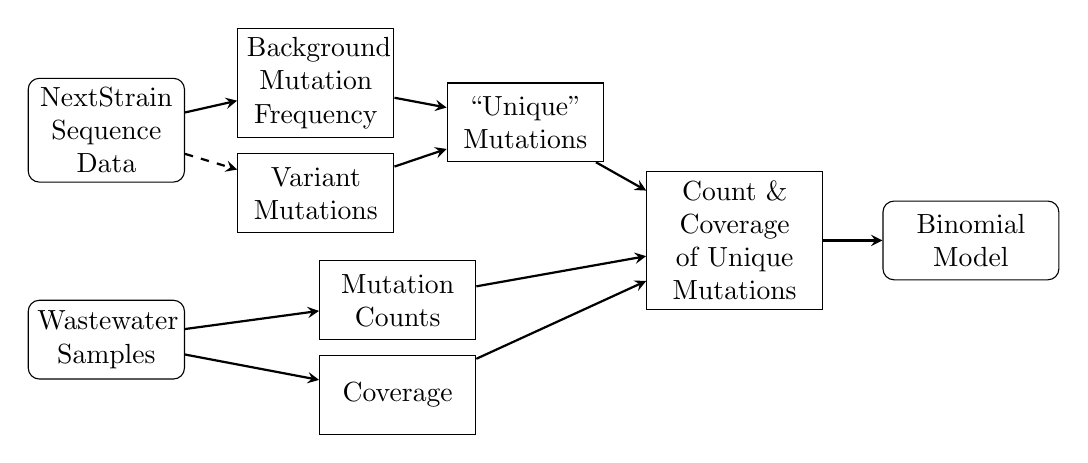
\begin{tikzpicture}[node distance=1cm]
\node (nextstrain) [startstop, text width=1.75cm] {NextStrain Sequence Data};
\node (nsmut) [process, right of=nextstrain, xshift=1.66cm, text width=1.75cm, yshift=0.6cm] {Background Mutation Frequency};
\node (nsomi) [process, below of=nsmut, text width=1.75cm, yshift=-0.4cm] {Variant Mutations};
\draw [arrow] (nextstrain) -- (nsmut);
\draw [thick, dashed,->,>=stealth] (nextstrain) -- (nsomi);

\node (waste) [startstop, below of=nextstrain, yshift=-1.66cm, text width=1.75cm] {Wastewater Samples};
\node (wmut) [process, right of=waste, xshift=2.7cm, yshift=0.5cm, text width=1.75cm] {Mutation Counts};
\draw [arrow] (waste) -- (wmut);
\node (wcov) [process, below of=wmut, yshift=-0.2cm, text width=1.75cm] {Coverage};
\draw [arrow] (waste) -- (wcov);

\node (uniques) [process, right of=nsmut, yshift=-0.5cm, xshift=1.66cm, text width=1.75cm] {``Unique'' Mutations};
\draw [arrow] (nsmut) -- (uniques);
\draw [arrow] (nsomi) -- (uniques);

\node (detect) [process, right of=uniques, yshift=-1.5cm, xshift=1.66cm, text width=2cm] {Count \& Coverage of Unique Mutations};
\draw [arrow] (uniques) -- (detect);
\draw [arrow] (wmut) -- (detect);
\draw [arrow] (wcov) -- (detect);

\node (model) [startstop, right of=detect, xshift=2cm, text width=2cm] {Binomial Model};
\draw [arrow] (detect) -- (model);

\end{tikzpicture}
\caption{The structure of our pipeline. NextStrain data are used to find the frequency of all mutations, then this is compared to the mutations of the variant (the dashed line indicates that this may or may not come from the NextStrain data) in order to find which mutations are common in the variant but uncommon in the population (``Unique'' Mutations). The wastewater samples are processed to determine which mutations are present and determine the number of times each position was observed (i.e., the coverage). The number of observations of the unique mutations is found, along with the coverage at the position of those mutations (the coverage is found regardless of whether that mutation was observed). Finally, a binomial model is used to estimate the proportion.}
\end{figure}


\section{Data Processing}

\subsection{Input Format}

% Context of data
Our pipeline assumes that data come from wastewater samples processed according to the ARTIC pipeline \cite{needed} on the Illumina NGS platform \cite{needed}, although the pipeline can be modified for other platforms.
The expected format is a FASTQ file \cite{needed}, where each entry represents one short read from the amplicons specified in ARTIC V3. TODO: Does it have to be V3? We didn't end up using the amplicons anywhere.
These files are expected to follow the FASTQ specification, with a sequence information row, the sequence itself, a plus sign, then the Phred score \cite{needed}.
A reference genome is also required for data processing.
We use Wuhan-1 \cite{needed} as the default, but the pipeline allows for specification by the user.



\begin{tightemize} 
    \item Required modifications for other platforms
\end{tightemize}

\subsection{Parsing FASTQ files}

% Description of desired output format
The purpose of this step of the pipeline is to convert the input FASTQ files into a list of mutations for each read and the coverage at each position of the reference genome.
The mutation list allows us to search for the mutations that we are interested in.
For a mutation that was not observed in the data, the coverage at each position allows us to determine whether it wasn't observed because there was low or zero coverage at the position where it would be or if there was sufficient coverage to detect it but it wasn't present.
The \texttt{minimap2.py} script accepts a FASTQ file (or pair of FASTQ files for paired-end reads) as well as a reference genome and outputs \texttt{mutations.csv} and \texttt{coverage.csv}.

% Parsing into features by mapping to reference
The \texttt{mutations.csv} file contains the mutation description, the position, and the coverage at that position.
The mutation description includes the alteration relative to the reference, which is labelled as \texttt{$\sim$}, \texttt{+}, or \texttt{-} for polymorphism, insertion, or deletion, respectively.
For polymorphisms, the nucleotide from the reference genome is not included in the label but the new nucleotide is.
For insertions, the added nucleotides are listed.
For deletions, the number of deletions is recorded.
If applicable, the 
This structure is demonstrated below.

%TODO: Get verbatim next to each other, with captions: https://stackoverflow.com/questions/2983839/latex-two-captioned-verbatim-environments-side-by-side
%TODO: anonymize 
\begin{verbatim}
position,label,mutation,frequency,coverage
27484,~27485C,aa:orf7a:L31S,0.00010871759827294332,64387
27484,~27485A,aa:orf7a:L31*,0.0002484973674810133,64387
\end{verbatim}

\begin{verbatim}
position,coverage
0,0
1,0
2,0
3,1
4,40
\end{verbatim}


\begin{tightemize}
    \item Dealing with paired-end data: mutations in one or both
    \item Dealing with paired-end data: coverage
    \item Calculating mutation frequency and coverage
    \item Implementation in \texttt{minimap2.py} (which is adapted from \texttt{covizu})
    \item Summary of output format and current implementation with \texttt{autoprocess.py}
\end{tightemize}

\begin{figure}[ht!]
\vspace{2cm}
\centering
\emph{Diagram: Two or three pairs in a FASTQ file, including some low quality score bases $\rightarrow$ Aligned to reference(including coverage) $\rightarrow$ Features and Coverage}
\vspace{2cm}
\caption{Extracting features from paired-end FASTQ files.}
\label{fig:feature_diagram}
\end{figure}

\subsection{Mutation Frequency}


\begin{tightemize}
    \item Motivation for getting this data
\end{tightemize}

\subsubsection{Background Frequency}
\begin{tightemize}
    \item Motivation for getting this data
    \item Accessing and processing GISAID data into mutations lists
    \item Calculating background frequencies (per-variant)
\end{tightemize}

\subsubsection{Variant-Specific Mutations}

\begin{tightemize}
    \item Obtaining mutations present in a variant from \texttt{minimap2} (noting that they are not enough to uniquely determine that variant))
    \item Obtaining mutations from PANGO when GISAID is not quite labelled right
    \item Comparison of background frequency to mutations (Omicron(95, 5)). 
    \item Including sub-lineages
\end{tightemize}

\begin{figure}[ht!]
\vspace{2cm}
\centering
\emph{Scatterplot of background frequency versus omicron frequency, coloured according to Omicronians(95,5), possibly with different shapes to denote the sub-lineages.}
\vspace{2cm}
\caption{Frequency of mutations in all variants versus in one specific variant. By comparing these two frequencies, we are able to specify variants that should only be common in our variant of interest.}
\label{fig:mutation_frequency}
\end{figure}






\section{Single Variant Detection}

\begin{tightemize}
    \item Motivation for Binomial GLMs
    \item Description of Binomial GLMs (incl. confidence intervals)
    \item Conservative 1\% sequencing error as our null hypothesis; not testing boundary of parameter space.
    \item Batch processing of GLMs
    \item Sensitivity analysis (using multiple definitions of variant-specific mutations, e.g. Omicronian(90, 10)).
\end{tightemize}






\section{Example Usage}

\begin{tightemize}
    \item Description of our particular data collection methods and project goals
    \item With permission, description of the results for Omicron in samples with good metadata.
\end{tightemize}

\begin{figure}[ht!]
\vspace{2cm}
\centering
\emph{Bar plots with confidence bands for GLM results, ordered by time.}
\vspace{2cm}
\caption{Results of the binomial GLM on our available data. The proportion of observed Omicron mutations appears to have increased slightly over time, but still does not reach the 1\% proportion required for us to confidently assert the presence of Omicron.}
\label{fig:binomial_results}
\end{figure}


\section{Discussion and limitations}

\begin{tightemize}
    \item The method is statistically good.
    \item The method is practically good.
    \item Can be modified to different wastewater data formats.
    \item We cannot detect unknown variants with this method.
\end{tightemize}


\bibliography{methods_bib}{}
\bibliographystyle{abbrvnat}

\end{document}

